%%%%%%%%%%%%%%%%%%%%%%%%%%%%%%%%%%%%%%%%%
% University/School Laboratory Report
% LaTeX Template
% Version 4.0 (March 21, 2022)
%
% This template originates from:
% https://www.LaTeXTemplates.com
%
% Authors:
% Vel (vel@latextemplates.com)
% Linux and Unix Users Group at Virginia Tech Wiki
%
% License:
% CC BY-NC-SA 4.0 (https://creativecommons.org/licenses/by-nc-sa/4.0/)
%
%%%%%%%%%%%%%%%%%%%%%%%%%%%%%%%%%%%%%%%%%

%----------------------------------------------------------------------------------------
%	PACKAGES AND DOCUMENT CONFIGURATIONS
%----------------------------------------------------------------------------------------

\documentclass[
	letterpaper, % Paper size, specify a4paper (A4) or letterpaper (US letter)
	11pt, % Default font size, specify 10pt, 11pt or 12pt
]{CSUniSchoolLabReport}

\usepackage{subcaption}
\usepackage{booktabs}
\geometry{top=2cm} % Override top margin to reduce space before title

%----------------------------------------------------------------------------------------
%	REPORT INFORMATION
%----------------------------------------------------------------------------------------

\title{Lab 1 - Electric Field  \\ ECE106} % Report title

\author{Yiran \textsc{Liu} \&  Zijin \textsc{Yang}} % Author name(s), add additional authors like: '\& James \textsc{Smith}'

\date{\today} % Date of the report

%----------------------------------------------------------------------------------------

\begin{document}

\maketitle % Insert the title, author and date using the information specified above

\begin{center}
	\begin{tabular}{l r}
      Lab Section: 206 \\
      Student Number: Y.L. 21184901 \& Z.Y. 21196273
	\end{tabular}
\end{center}
%----------------------------------------------------------------------------------------
%	COMPUTATIONS
%----------------------------------------------------------------------------------------

\section{Hand Computations}

\subsection{Electric field of a single point charge}

A point charge of $+1\mu C$ is placed at $(x, y, z) = (0, 0, 0)$, we can compute that the electric field at the following three coordinates using the equation:
\[
  \vec{E} = \frac{1}{4\pi\epsilon_{0}} \frac{q}{r^2}\hat{r}
\]
where $\epsilon_{0} = 8.854187 \times 10^{-12} \ F / m$ and $q = 1.0 \times 10^{-6} C$

\begin{enumerate}
  \item At $\vec{r} = (0.2, 0, 0)$, we have 
    \[
      \vec{E} = \frac{1}{4 \pi \epsilon_{0}} \frac{1.0 \times 10^{-6}}{0.2^2} \hat{i} = (224689, 0, 0)
    \]
  \item At $\vec{r} = (0.4, 0, 0)$, we have 
    \[
      \vec{E} = \frac{1}{4 \pi \epsilon_{0}} \frac{1.0 \times 10^{-6}}{0.4^2} \hat{i} = (56172.2, 0, 0)
    \]
  \item At $\vec{r} = (0.6, 0, 0)$, we have 
    \[
      \vec{E} = \frac{1}{4 \pi \epsilon_{0}} \frac{1.0 \times 10^{-6}}{0.6^2} \hat{i} = (24965.4, 0, 0)
    \]
\end{enumerate}


\subsection{Volume Charge Density Calulation}

To compute the volume charge density of a sphere with $r=0.01m$ and uniform distributin of its $+1\mu C$ charge (or $+1 \times 10^{-6}$), we first compute the volume:
\[
  V = \frac{4}{3} \pi r^3 = 4.18879 \times 10^{-6} \ m^{3}
\]
\[
  \rho = \frac{q}{V} = 0.238732 \ C \cdot m^{-3}
\]



%----------------------------------------------------------------------------------------
%	SIMULATION RESULTS ANALYSIS
%----------------------------------------------------------------------------------------

\section{COMSOL Results Analysis}

Following the lab instructions, we created this physics simulation of a sphere charge of $r=0.01m$ and uniform charge density $\rho=0.238732 \ C \cdot m^{-3}$ and three observation points at $(0.2, 0, 0), (0.4, 0, 0) and (0.6, 0, 0)$, assuming electrical potential $\phi = 0V$ at $R=6m$. 

\begin{figure}[H] % [H] forces the figure to be placed exactly where it appears in the text
	\centering % Horizontally center the figure
	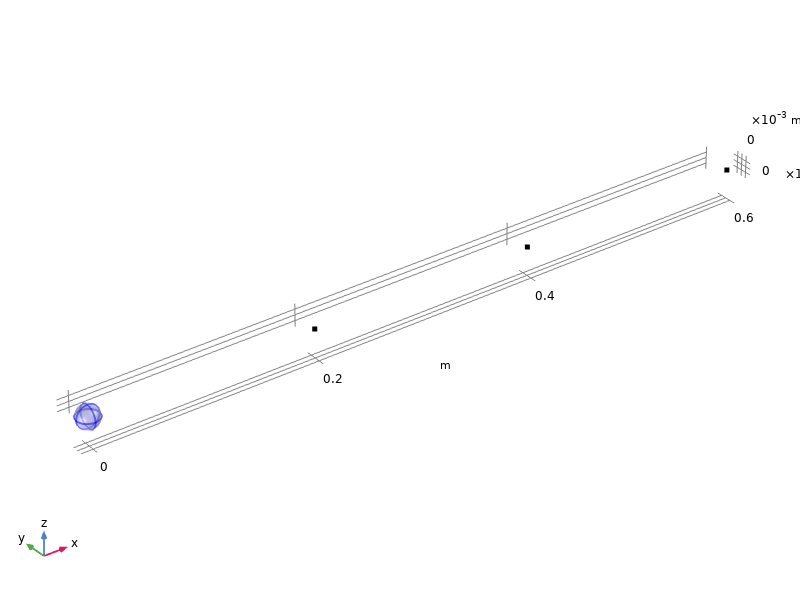
\includegraphics[width=0.9\textwidth]{./Figures/Overview.png} % Include the figure
	\caption{Overview of simulation setup, boundary sphere not shown.}
\end{figure}

\subsection{Electric Potential}

Plotting the electric field potential at default view, we observe no significant change in the entire space ($R=6m$) since this space is too big. Zooming in, we see that electric potential decreases rapidly as distance from charge increases. 

\begin{figure}[H]
    \centering
    \begin{subfigure}[b]{0.48\textwidth}
        \centering
        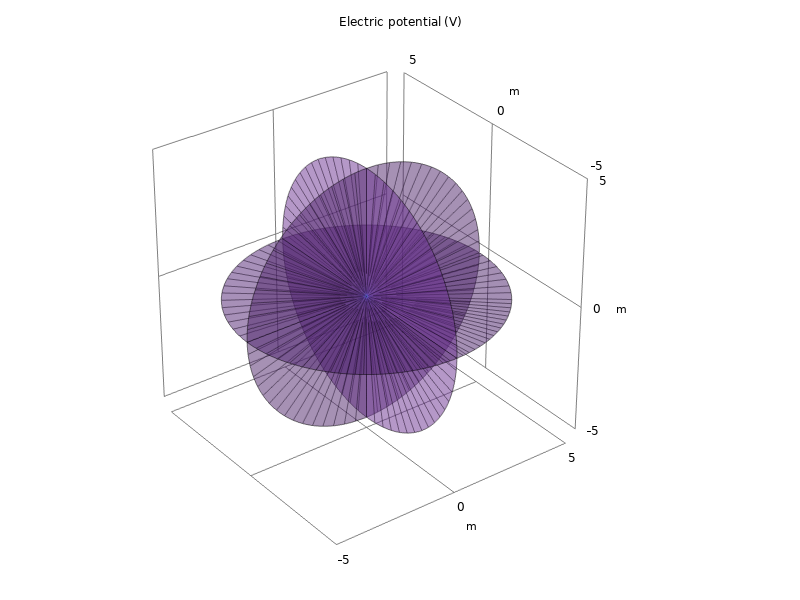
\includegraphics[width=\linewidth]{./Figures/Potential-Default.png}
    \end{subfigure}
    \hfill
    \begin{subfigure}[b]{0.45\textwidth}
        \centering
        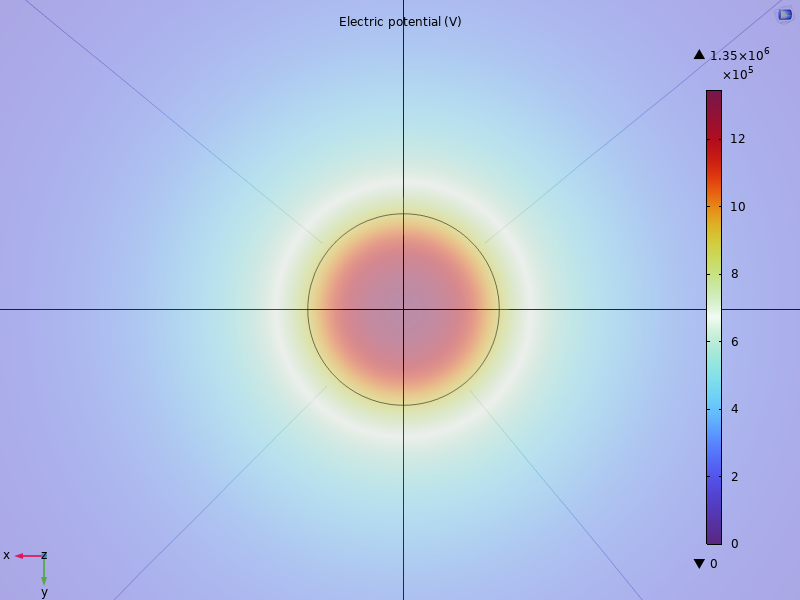
\includegraphics[width=\linewidth]{./Figures/Potential-2D.png}
    \end{subfigure}
    \caption{Electric field potential heatmaps. (Left) Multislice plot of the entire boundary space at \textit{Default View}; (Right) 2D plot of space near the sphere charge.}
\end{figure}

\subsection{Electric Field}

We plot the electric field and observe an inverse square relationship between distance and electric field strength, with Electric field direction pointing outwards from the charge. 

\begin{figure}[H] % [H] forces the figure to be placed exactly where it appears in the text
	\centering % Horizontally center the figure
	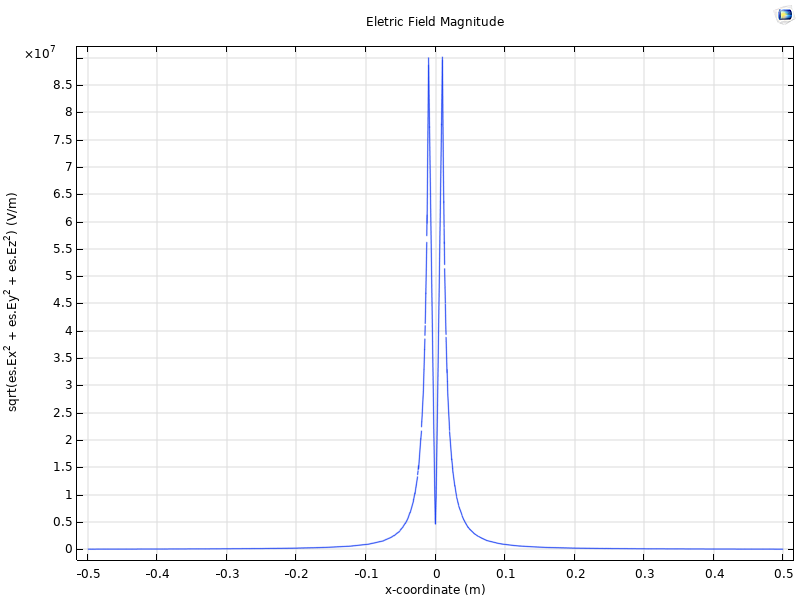
\includegraphics[width=0.75\textwidth]{./Figures/Electric Field Magnitude.png} % Include the figure
  \caption{Electric Field Magnitude near the source charge.}
\end{figure}

\begin{figure}[H] % [H] forces the figure to be placed exactly where it appears in the text
	\centering % Horizontally center the figure
	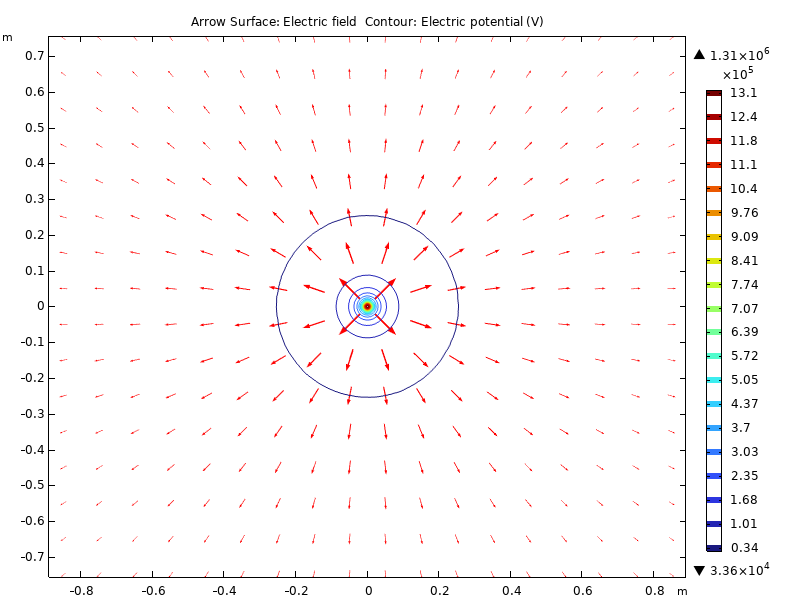
\includegraphics[width=0.75\textwidth]{./Figures/Electric Field with Contour.png} % Include the figure
	\caption{Electric Field with Contour.}
\end{figure}

\subsection{Comparison with Theoretical Value}

We compare the computed electric field strength with theoretical value and found the result to be in an acceptable range of error.

\begin{table}[H]
    \centering
    \caption{Comparison of simulated electric field strength with theoretical predictions at three observation points.}
    \label{tab:electric_field_comparison}
    \begin{tabular}{lcrr}
        \toprule
        \textbf{Distance (m)} & \textbf{Simulated (V/m)} & \textbf{Theoretical (V/m)} & \textbf{\% Error} \\
        \midrule
        0.2 & 225139.5 & 224689.0 & 0.20 \\
        0.4 & 56114.6 & 56172.2 & 0.10 \\
        0.6 & 25292.7 & 24965.4 & 1.31 \\
        \bottomrule
    \end{tabular}
\end{table}
%----------------------------------------------------------------------------------------
%	ENHANCEMENT ACTIVITY
%----------------------------------------------------------------------------------------

\section{Enhancement Activity}
We build the model of three source charges and one measuring point according to the description.

\begin{figure}[H] % [H] forces the figure to be placed exactly where it appears in the text
	\centering % Horizontally center the figure
	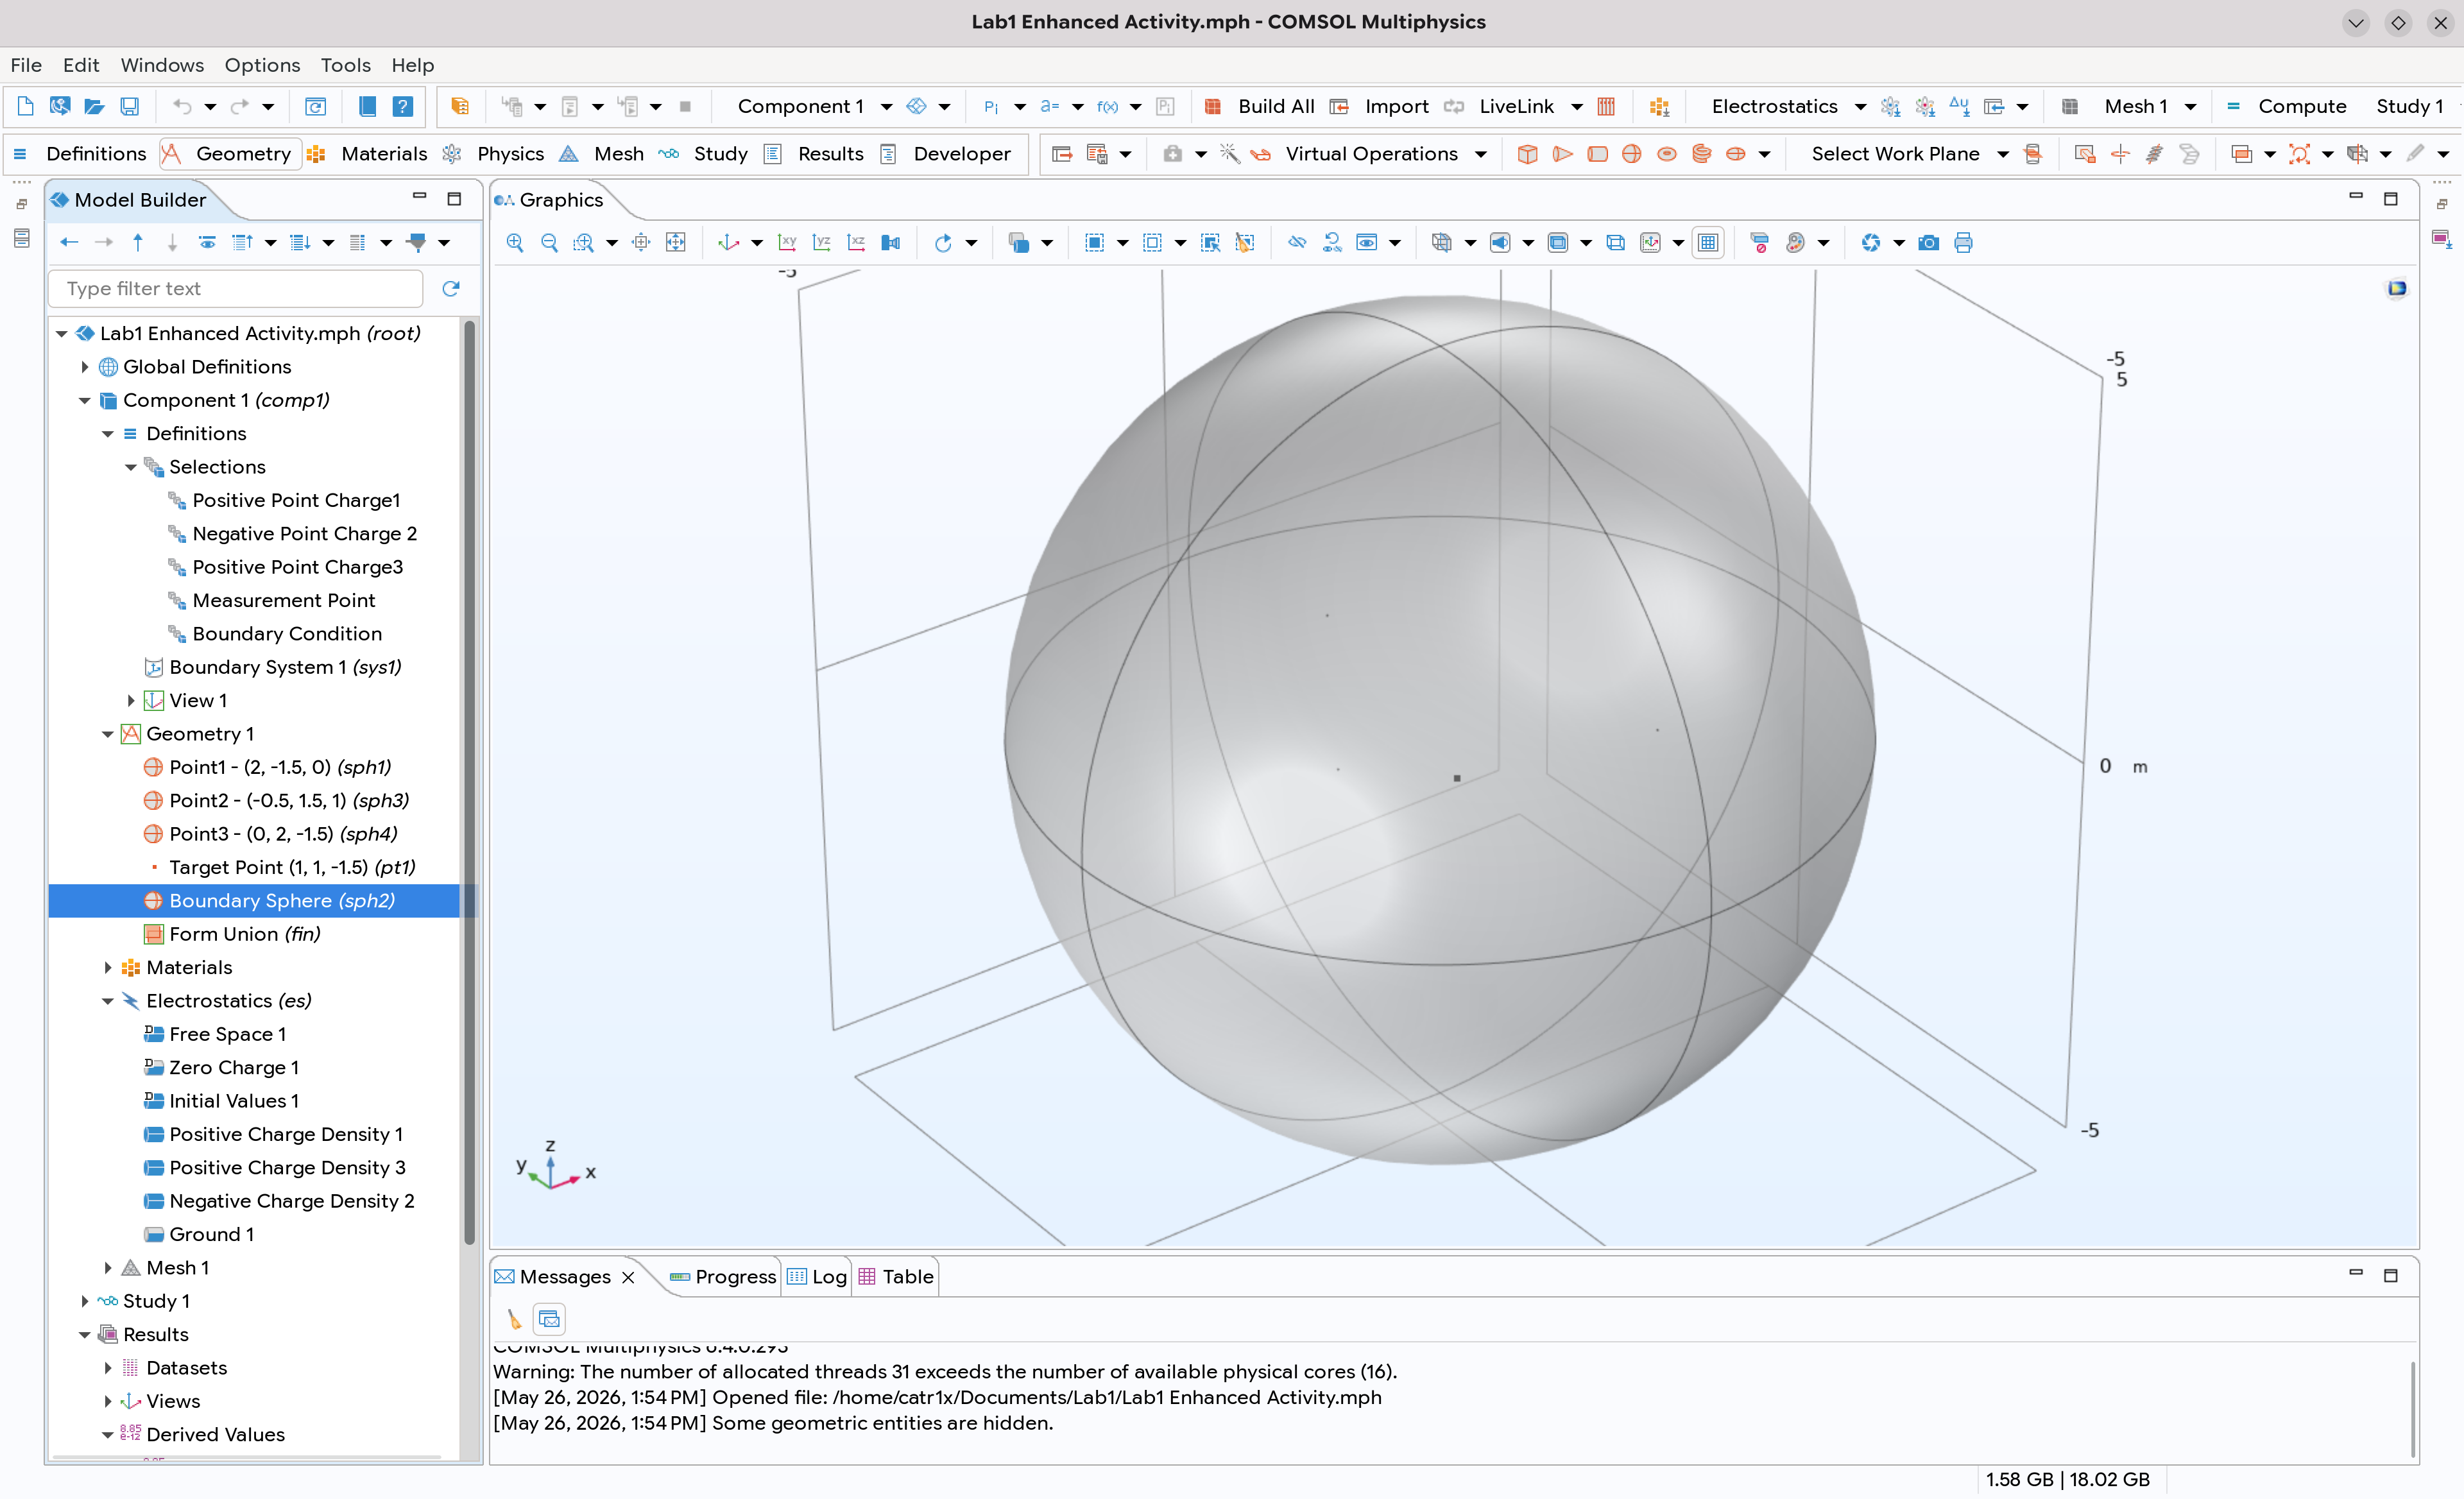
\includegraphics[width=\textwidth]{./Figures/Enhancement Activity.png} % Include the figure
  \caption{Screenshot of COMSOL model.}
\end{figure}


We find that the electric field strength and the observation point $(1.0, 1.0, -1.5)$ is 

\[
\vec{E} = (2481.5, -2233.2, 220.07) \ N/C
\]

Using Columnb's law, the force experienced by the charge is 
\[
\vec{F_e} = q \vec{E} = (0.0024815, -0.0022332, 0.00022007) \ N 
\]

\end{document}
